\chapter{System Design}

In this chapter the project is further analysed, by providing diagrams 
and describing basic notions, setting up the premises for implementing
the ARINC 653 standard.

\section{System Overview}
As a means to both explaining the system and as a practical development
model, the system can be thought of as being made up of layers.
Each layer being an abstraction of workings in the layers beneath it,
with the partitions at the top and the hardware at the bottom.
This model is defined by the ARINC 653 standard
and expanded upon here with drivers being build on top of the HAL library,
instead of directly on top of the hardware,
creating an extra layer of abstraction.
\todo{link with figure}

\begin{itemize}
	\item \textbf{Partitions}
		are independent program units that contain applications. These
		applications can in turn interact with other systems. The
		partitions are achieving this  in complete isolation from 
		one another.
	\item \textbf{APEX}
		defines the methods by which the partitions talk to the world and
		interact with other partitions or the OS, running
		on the same core module or connected to other ARINC systems.
	\item \textbf{OS}
		provides the infrastructure for partitions to operate. This 
		includes their scheduling, message passing and processes 
		the APEX calls.
	\item \textbf{Drivers}
		define the way the hardware should run.	
		They serve the OS with methods to create an environment in which
		partitions can be run and scheduled without influencing one
		another.
	\item \textbf{HAL and CMSIS}
		are hardware abstraction layers that make setting up the hardware
		easier for developers. HAL is provided by the chip manufacturer - 
		STMicroelectronics. CMSIS is provided by ARM the company that
		developed the chip architecture.
	\item \textbf{Hardware}
		is the physical platform on which everything is executed. This 
		includes the actual CPU and its peripherals.
\end{itemize}

\todo[inline, color=green]{An XML file is provided by the system developer
 at compile time.It defines how the top layers interact and set the
  requirements of the drivers and the underlying hardware.
Every layer contains a list of components, which provides the
 functionalities of that layer.
Beneath graphical overview of the different layers with their core
 components is provided.}
 
\begin{figure}[H]
\centering
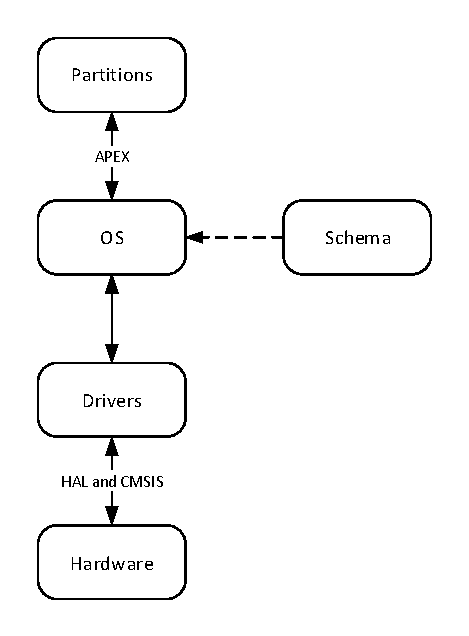
\includegraphics[width=4cm,keepaspectratio]{simple_system_architecture.pdf}
\captionof{figure}{A simple system overview}
\end{figure}

In the rest of the chapter the different layers are described,
from bottom up, 
together with their core components.The hardware specifications
are outlined, as well as explaining how the system is initialised.

\subsection{Hardware}
As mentioned in the previous chapter, the hardware used for this project 
is a MINI-M4 board from MikroElectronica. This is build around an
STM32F415RG microcontroller produced by STMicroelectronics. Besides
this, the board contains two crystal oscillators, two LEDs, a reset 
button and the peripherals for supplying power via a microUSB connector.
Some of the GPIOs are break through using external pins.
\todo{REFERENCes, referenes} 
These pins were soldered to the board, and this was setup on a breadboard
for practicality, as seen in \ref{fig:photo1}.

\begin{figure}[H]
\begin{subfigure}{0.5\textwidth}
  \centering
  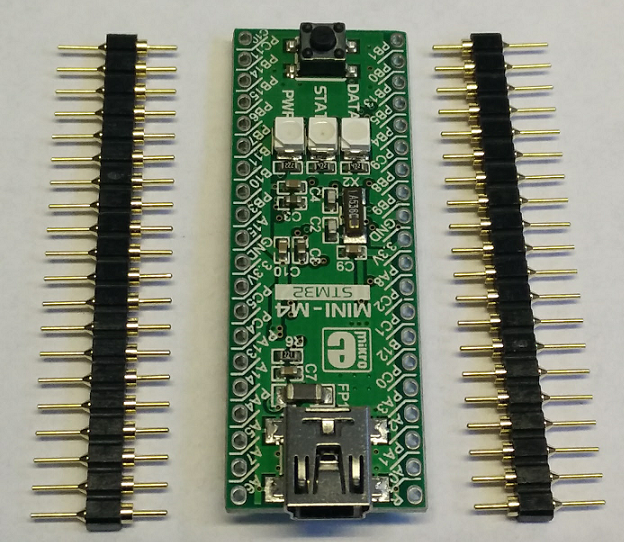
\includegraphics[width=3cm]{hardware/board_not_soldered.png}
  \caption{MINI-M4 before soldernig}
  \label{fig:sub1}
\end{subfigure}%
\begin{subfigure}{0.5\textwidth}
  \centering
  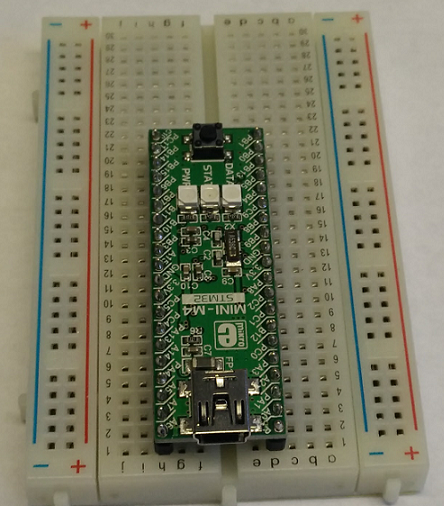
\includegraphics[width=3cm]{hardware/board_on_breadboard.png}
  \caption{MINI-M4 on a breadboard}
  \label{fig:sub2}
\end{subfigure}
\caption{Preparation of the board}
\label{fig:photo1}
\end{figure}

For programming and debugging the board the JTAG interface was used.
This had to be connected to certain pins of the board. In order to get 
feedback from the board, a serial connection was used, which requires two
more lines to it. This can be seen in the next figure.

\begin{figure}[H]
\centering
\begin{subfigure}{.5\textwidth}
  \centering
  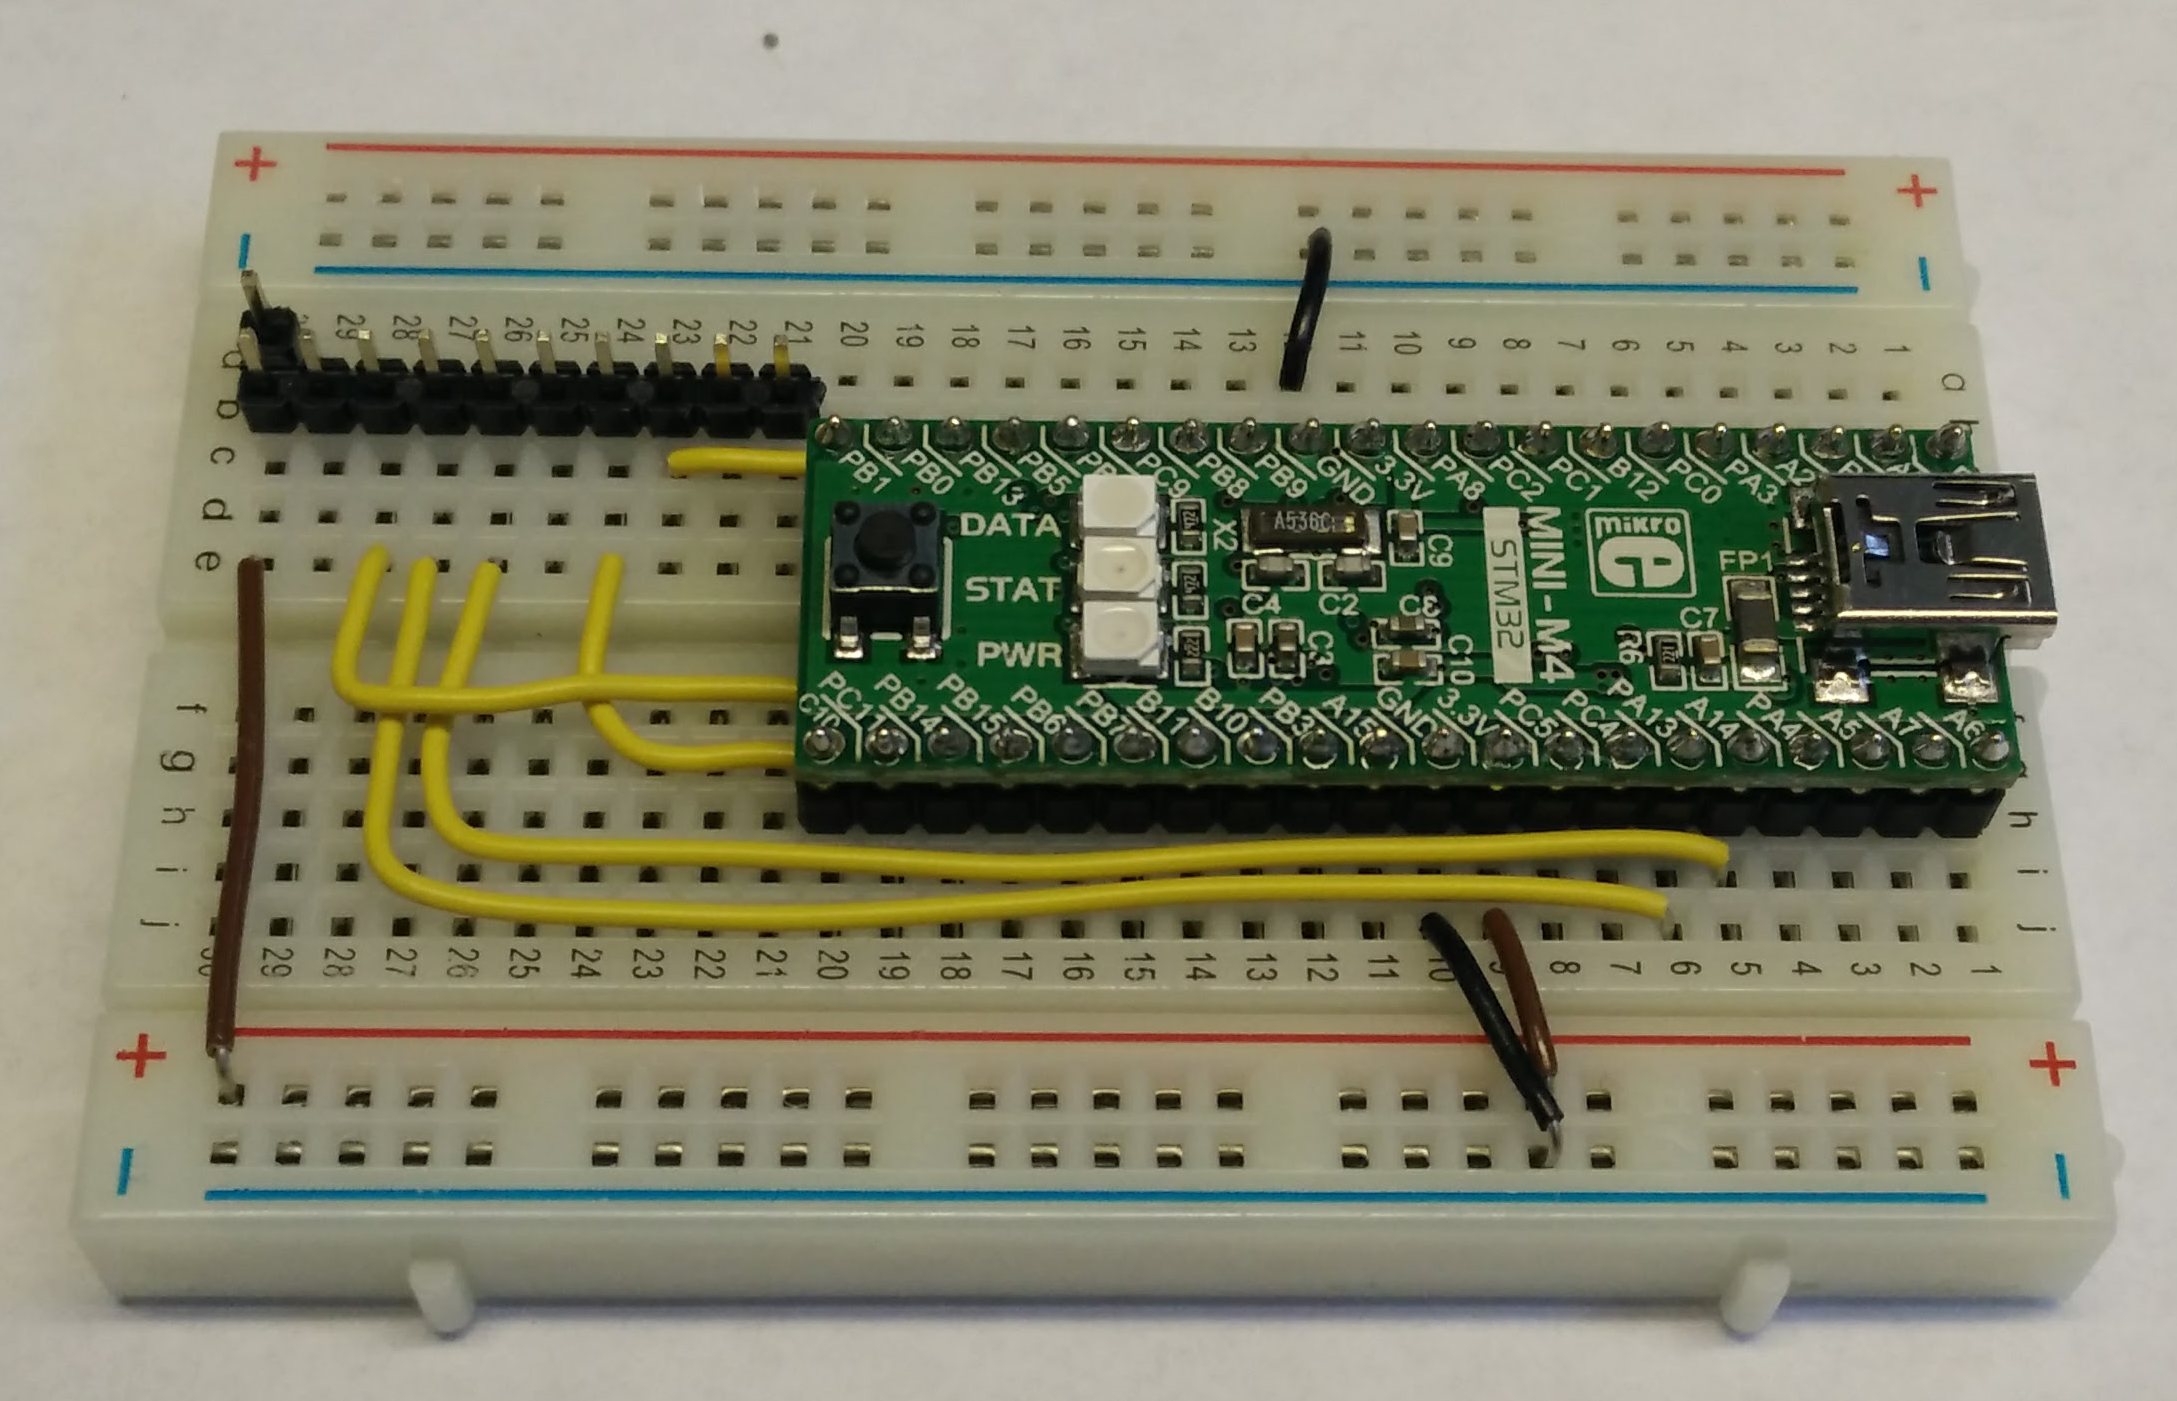
\includegraphics[width=.4\linewidth]{hardware/board_with_jtag_lines}
  \caption{The JTAG lines}
  \label{fig:sub1}
\end{subfigure}%
\begin{subfigure}{.5\textwidth}
  \centering
  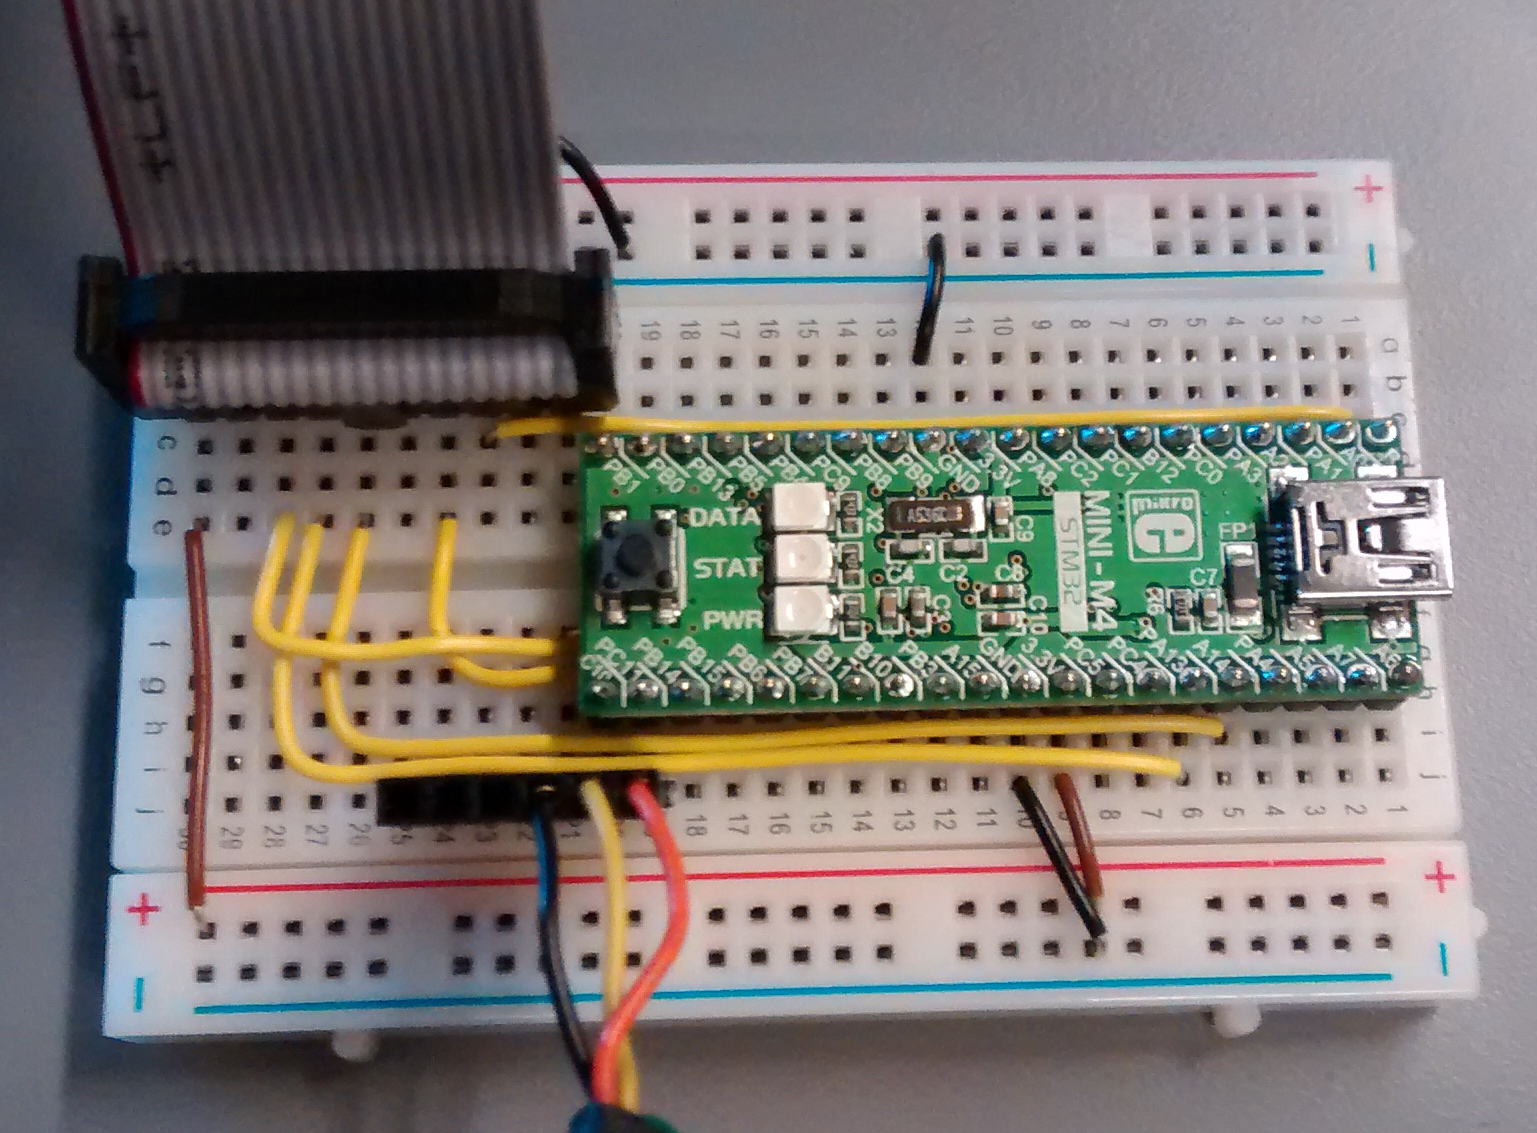
\includegraphics[width=.4\linewidth]{hardware/board_with_jtag_and_serial}
  \caption{Both the JTAG and serial interfaces}
  \label{fig:sub2}
\end{subfigure}
\caption{Connecting the board}
\label{fig:photo2}
\end{figure}

After this, the board was ready to be used in the development process.
The only drawback of this setup, is that it requires three USB ports:
power for the board, the JTAG interface, and the serial communication.

\subsection{HAL and CMSIS}
These two libraries are truly the workhorse when dealing with the 
board\textquotesingle s peripherals. Basically, the CMSIS library
is defining the data structure and address mapping on all peripherals.
This means that the HAL library can then use these definitions for its
utilities in a more straightforward way. Besides this, CMSIS handles
all the exceptions occurring in the chip, and the HAL library configures
the interrupts.
\todo{IS this understandable?}
 
\begin{figure}[H]
\centering
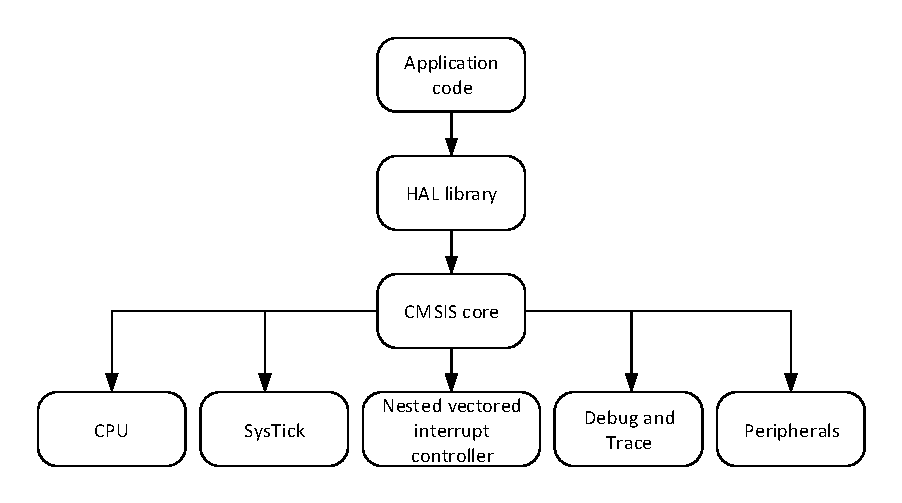
\includegraphics[width=\linewidth,keepaspectratio]{HAL_CMSIS.pdf}
\captionof{figure}{The structure of the libraries}
\end{figure}
\todo[inline, color=green]{do i need reference for this figure?
\url{<http://www.keil.com/pack/doc/CMSIS/General/html/CMSISv4_small.png>}
}
\subsection{Drivers}
\todo{this kind of lists do not fit very well the purpose}
\begin{description}[align=left]
	\item [\textbf{UART driver}] The UART is used by the system to communicate with the outside
	world. This can either receive or transmit data to another UART device.
	\item [\textbf{Watchdog timer driver}] The watchdog timer is necessary to ensure recovery
	in case of a hardware fault or program error. If this happens, the program would be restarted
	from a safe state.
	\item [\textbf{LEDs}]The LEDs are mainly used for debugging. They are
	are connected to two GPIO pins.
	\item [\textbf{System Clock}]The system clock needs to be initialised 
	in order to provide a clock source for the CPU and the peripherals.
	there is a multitude of choices, ranging from internal or external
	oscillators, to high or low speed crystals. Besides this, certain
	peripherals can use their own, individual clock source that also has
	to be configured.
	\item [\textbf{RTC}]This is the real time clock implemented in the 
	chip. The purpose of this is to keep track of time accurately. This 
	is why it uses a 32,768kHz oscillator as a clock source, which is 
	the standard in the field.
	\item [\textbf{MPU}]The Memory protection unit is required by the
	ARINC 653 standard, since the system should have a way to manage its
	memory.
	\item [\textbf{Delay}]This is just a simple function, based on a call
	for another function from the HAL library. It delays the execution 
	of the program by a factor of milliseconds.
	\item [\textbf{Timing}]This driver has the purpose to keep track of 
	relative time. As the standard specifies, it should be counting in 
	nanoseconds.

\end{description}

\subsection{OS}
\subsubsection{Scheduler}
A scheduler decides which process should be executed by the processor available, according to some rules. In this implementation we have 2 levels of scheduling, one to switch between partitions and a second one for processing the processes of each partition.

For the first one we used a Manual Scheduler, that gives a certain amount of time of processor to each partition, according to its demand and importance. Those values can't be changed in running time, following the same rules during the whole execution. Every milisecond we verify if the time of the partition running has reached the timeout, if so, we switch the context for the next partition. And the new partition gets the processor.

The second one is a Pre-emptive Priority Scheduler, based on the processes' priority, in which is executed the one with the highest priority until it loses the processor to other partition. Every milisecond we pick the process, from the array of processes of that partition, with the highest priority and run in the processor.

\paragraph{Context switching} is to switch from executing one block of code $b_1$ to another block of code $b_2$
with the intend to eventually return to $b_1$ in a way that is transparent to the blocks of code.
This allows for code to be partitioned into separate independent blocks that can run concurrently.
This is opposed to monolithic blocks of code that entirely control the flow of execution.
Therefore, context switching is essential for any operating system that wishes to utilise a scheduler to allow concurrent execution of code.
Context switching works by saving the state of the CPU registers from one context to memory,
and then switching to another context by restoring the state of the registers previously saved in memory.
Since context switching must manipulate registers directly and individually, it is a feature that must be implemented
on a very low level of abstraction, and it can change significantly from one CPU architecture to another.
The scope of this project is to only implement an operating system for a Cortex M4. Hence context switching needs only
to work on the architecture used by this chip.\\
Context Switching on the Cortex M4 is partially handled by the Nested Vectored Interrupt Controller (NVIC).
When an exception (this includes interrupts) occurs, the NVIC will change context to an exception handler.
Upon changing context from regular code to the exception handler, the NVIC will save the registers R0-R3, R12, LR, PC and PSR
on the stack. These are only some of the registers. Why the decision was made to make the hardware save some of the
registers instead of letting software handle all, is unknown. \todo{Research harder the reason why the NVIC saves some register.}
When the exception handling routine exits, and control is handed back to the NVIC,
the NVIC will restore these registers again.\\
If the operating system wishes to switch context, it must save the remaining registers, R4-R11, and the stack pointer to memory
pick a new context to restore, reload the registers R4-R11 and the stack pointer of the new context from memory,
and hand back control to the NVIC. The NVIC will then reload the remaining registers from the stack of the new context. To see a figure of the registers and who saves them, see figure \ref{tab:registers}\\\\
\begin{table}[H]
	\centering
	\begin{tabular}{|c|c|p{9.5cm}|}
		\hline
		Register	&	Saved by	&	Purpose\\
		\hline
		R0			&	Hardware	&	General purpose (Argument value + return value)\\
		\hline
		R1-R3		&	Hardware	&	General purpose (Argument value)\\
		\hline
		R4-R11		&	Software	&	General purpose (Local variable)\\
		\hline
		R12			&	Hardware	&	General purpose (Intra-Procedure-call scratch)\\
		\hline
		R13 (SP)	&	Software	&	Stack pointer [Banked]\\
		MSP			&	Software	&	Master stack pointer (Stack pointer for kernel space)\\
		PSP			&	Software	&	Process stack pointer (Stack pointer for user space)\\
		\hline
		R14 (LR)	&	Hardware	&	Link register\\
		\hline
		R15 (PC)	&	Hardware	&	Program Counter\\
		\hline
		xPSR		&	Hardware	& 	Special-purpose Program Status Register\\
		\hline
	\end{tabular}
	\caption{A table of the CPU registers of a Cortex M4. Notice that register R13 (stack pointer) is banked;
	there are separate registers for user space and kernel space.
	For registers, aliases are written in parenthesis, and for purpose, calling convention is written in parenthesis.}
	\label{tab:registers}
\end{table}
As added complexity, the Cortex M4 utilises two different stack pointers, the Master Stack Pointer (MSP) and the Process Stack Pointer (PSP).
The MSP is intended for kernel space execution and the PSP is intended for user space execution, but there is no enforcement.
Switching between the two cannot be done in an exception handler, but must instead be done by the NVIC.
Since the path to the new context goes through the NVIC, the NVIC is also partially responsible setting the state of the processor.
This is done by loading an EXC\_RETURN value into the Program Counter. See table \ref{tab:exc-return} for the different values.
To make context switching transparent to the applications running, it's important that the state the processor returns to, is the
same it earlier came from. Therefore, upon entry into the interrupt routine, the NVIC loads the appropriate EXC\_RETURN into the Link
register. This value must be saved by software to assure it can return to the right state.
\begin{table}[H]
	\centering
	\begin{tabular}{|c|p{10cm}|}
		\hline
		Value			&	Description 	\\
		\hline
		0xFFFF FFF1 	&	Return to Handler mode, using the Master Stack Pointer, but without the floating point unit.	\\
		\hline
		0xFFFF FFF9		&	Return to Thread mode, using the Master Stack Pointer, but without the floating point unit.		\\
		\hline
		0xFFFF FFFD		&	Return to Thread mode, using the Process Stack Pointer, but without the floating point unit.	\\
		\hline
		0xFFFF FFE1		&	Return to Handler mode, using the Master Stack Pointer, with the floating point unit.			\\
		\hline
		0xFFFF FFE9		&	Return to Thread mode, using the Master Stack Pointer, with the floating point unit.			\\
		\hline
		0xFFFF FFED		&	Return to Thread mode, using the Process Stack Pointer, with the floating point unit.			\\
		\hline
	\end{tabular}
	\caption{
		A table of the possible EXC\_RETURN values. An interrupt service routine is exited by loading one of these values into the Program Counter register.	}
	\label{tab:exc-return}
\end{table}

\subsubsection{Interpartition communication}

\section{XML}


\section{Memory Management}
ARINC 653 advertises time and space separation covered in.
\todo[inline]{ref to sec in analysis}
To accommodate for the feature of separating partitions in space,
this operating system relies on the memory management unit (MPU)
to manage permissions across sections of memory,
ensuring that partitions stay within a dedicated memory space.

\subsection{something about ARINC on memory management}
The ARINC 653 standard OS, uses a statically allocated memory layout for everything
that gets compiled.
\todo[inline]{reference to standard}
This means that no memory allocation is permitted at runtime
outside predefined memory sections.
This policy ensures a fixed and predictable sandboxing environment, where partitions
can not restrict other parts of the system by occupying memory resources.
It also gives the system developer a way to ensure that the system has enough memory
for all processes to function correctly, given that this amount can be predetermined.

Memory regions are declared in the XML file, included at compile time, for a list
of different system features, like individual partitions and communication buffers.
All of this information is important for different reasons when setting up the system.
The rest of this section will deal with the subject of managing memory regions on a STM32F415 chip
and categorizing and analysing the memory requirements into a single memory strategy to implement in
\todo[inline]{ref to memory management implementation}.

\subsection{the MPU on a STM32F415}

\subsection{memory strategy}

\section{Conclusion - Discussion}

Figure \ref{fig:advanced_system} presents the system in its entirety,
with all the components organised in the corresponding layers.

\begin{figure}[H]
\centering
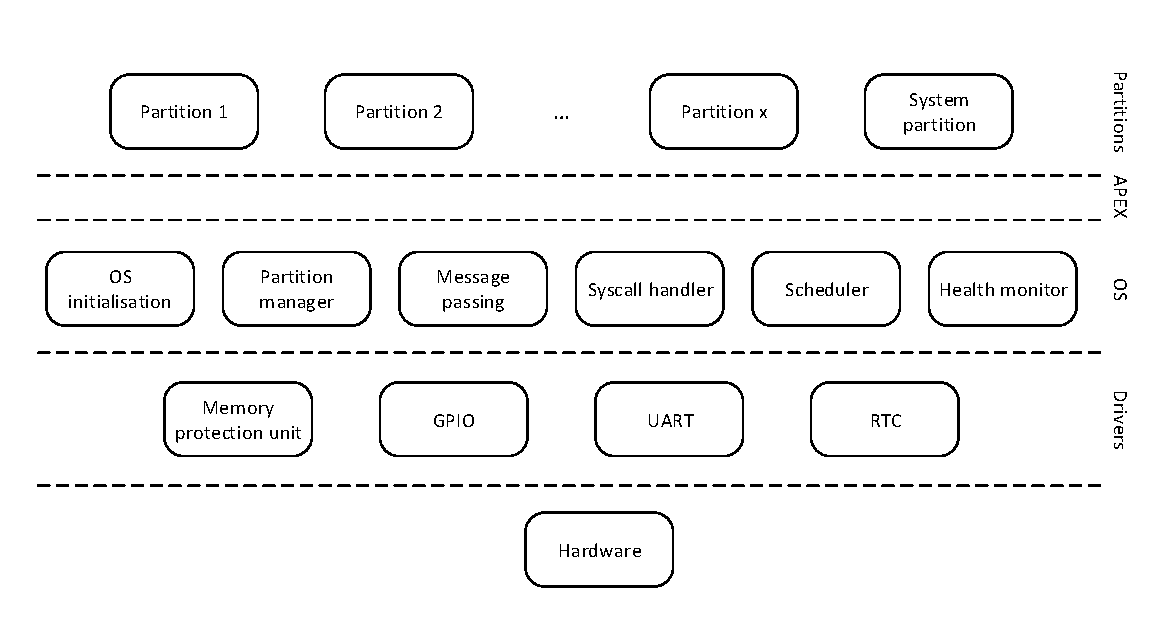
\includegraphics[width=\textwidth]{advanced_system_architecture.pdf}
\caption{An advanced system overview}
\label{fig:advanced_system}
\end{figure}

The following chapter will go through how all these components,
features and functionalities has been implemented.